%======================================================================
%\begin{frame}\frametitle{Scramjets}
%
%
%
%\begin{itemize}
%\item \sPI{scramjet} --- supersonic combustion ram jet  
%\begin{itemize}
%\setlength{\itemsep}{0.05in}
%
%  \item \rPI{Supersonic combustion}:  avoids
%    deceleration/compression losses
%    
%    
%  \item \rPI{Air-breathing}:  avoids weight penalty of onboard
%    oxidizer
%
%  \item[] \ldots nominally simple, but extreme conditions are challenging 
%\end{itemize}
%\end{itemize}
%
%\begin{center}
%\begin{minipage}{0.5\textwidth}
%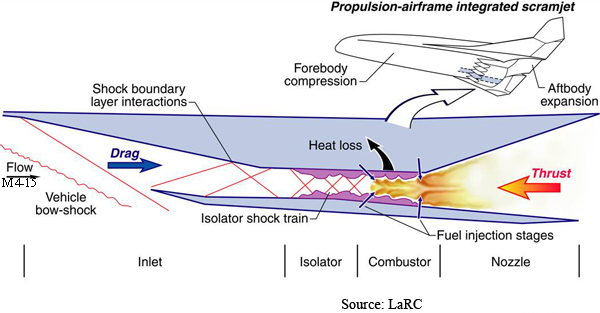
\includegraphics[width=\textwidth]{Figures/scramjet-LaRC.png}
%\end{minipage}
%\hfil
%\begin{minipage}{0.18\textwidth}
%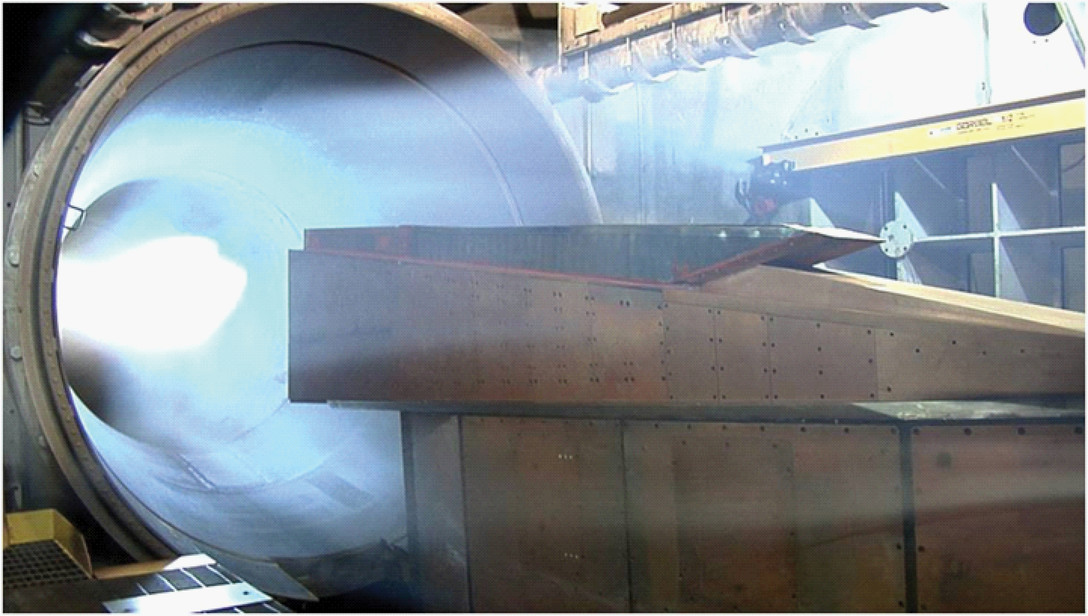
\includegraphics[width=\textwidth]{Figures/scramjet-groundtest.png}
%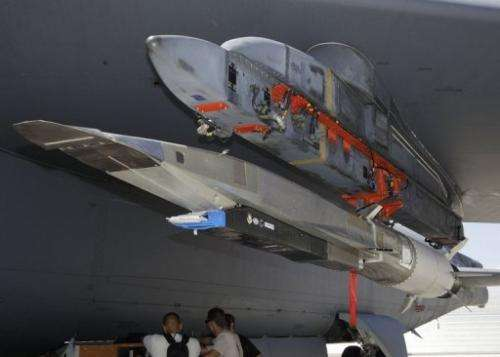
\includegraphics[width=\textwidth]{Figures/scramjet-launcher.png}
%\end{minipage}
%\begin{minipage}{0.18\textwidth}
%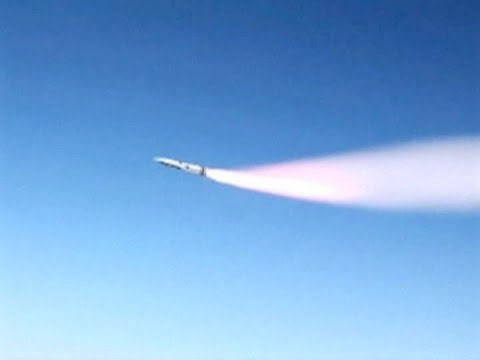
\includegraphics[width=\textwidth]{Figures/scramjet-x51a-flighttest.png}
%\end{minipage}
%\end{center}
%
%  \begin{itemize}
%
%  \item \rPI{Enables}:  access to space, global transport,
%    next-generation delivery systems
%
%\end{itemize}
%
%\end{frame}
%======================================================================


% %======================================================================
% \begin{frame}\frametitle{Core Technical Challenge}

% \begin{huge}
% \begin{center}
% \begin{tabular}{rc}
% Flow speed: & $\approx 2000\,\mathrm{m/s}$\\
% \\
% \\
% Laminar flame speed: & $\lesssim 10\,\mathrm{m/s}$
% \end{tabular}
% \end{center}
% \end{huge}

% \end{frame}
% %======================================================================


% %======================================================================
% \begin{frame}\frametitle{Follow-on Technical Challenges}

% \begin{minipage}{0.55\textwidth}
% \begin{itemize}
% \setlength{\itemsep}{0.2in}
% \item Scramjet:  conflicting goals
% \begin{itemize}
%   \item enough turbulence mixing for complete combustion
%   \item low enough loses to maintain internal supersonic flow
%   \item small changes in geometry matter:  efficiency and robustness
% \end{itemize}
% \item Thermal resistance 
% \begin{itemize}
%   \item combustion $\to$ high-$T$ \\\hfill $\to$ risks melt/burn 
%   \item high-$T$ $\to$ sustain combustion
%   \item strength required
% \end{itemize}
% \end{itemize}
% \end{minipage}
% \hfill
% \begin{minipage}{0.4\textwidth}
% 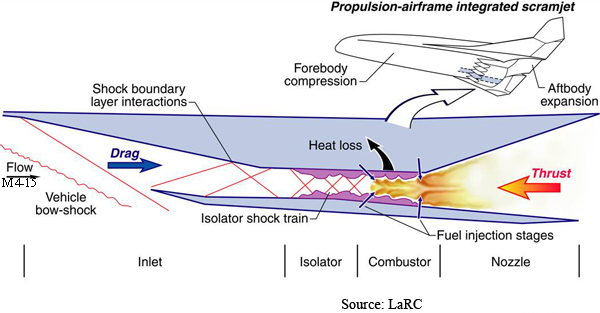
\includegraphics[width=\textwidth]{Figures/scramjet-LaRC.png}
% \vspace*{0.3in}

% 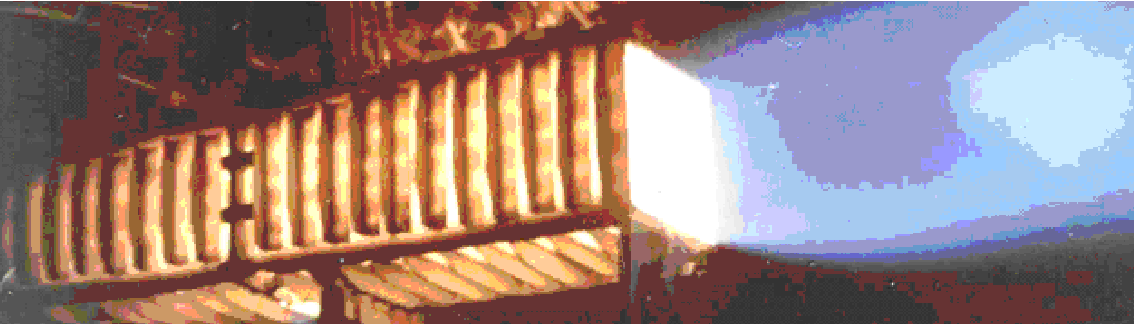
\includegraphics[width=\textwidth]{Figures/scramjet-niobium-russian.png}

% \begin{center}
% \begin{tiny} 
% ``Niobium scramjet''\par
% Moscow Aviation Institute\par
% \end{tiny}
% \end{center}
% \end{minipage}
% \medskip

% \begin{itemize}
% \item Weight saving compounded with fuel weight savings
% \end{itemize}

% \end{frame}
% %======================================================================


%======================================================================
%\begin{frame}\frametitle{Design Opportunity:  Advanced Composites}
%
%\vspace*{0.1in}
%
%\begin{minipage}{0.53\textwidth}
%\begin{itemize}
%\setlength{\itemsep}{0.15in}
%\item High-$T$, low-weight composites:
%\begin{itemize}
%\setlength{\itemsep}{0.1in}
%\item \textit{Dense} --- strong and heat resistant
%\item \textit{Porous} --- tailored thermal protection 
%\item \textit{Flexible} --- morphing for flight-regime robustness
%\end{itemize}
%
%\item Common features:
%\begin{itemize}
%\setlength{\itemsep}{0.1in}
%  \item Carbon-fiber:  weave or pack
%  \item Coatings or matrix ---\\\hfill ceramics, resins, phenolics, \ldots
%\end{itemize}
%\end{itemize}
%\end{minipage}
%\hspace*{-0.1\textwidth}
%\begin{minipage}{0.55\textwidth}
%\raisebox{0.3in}{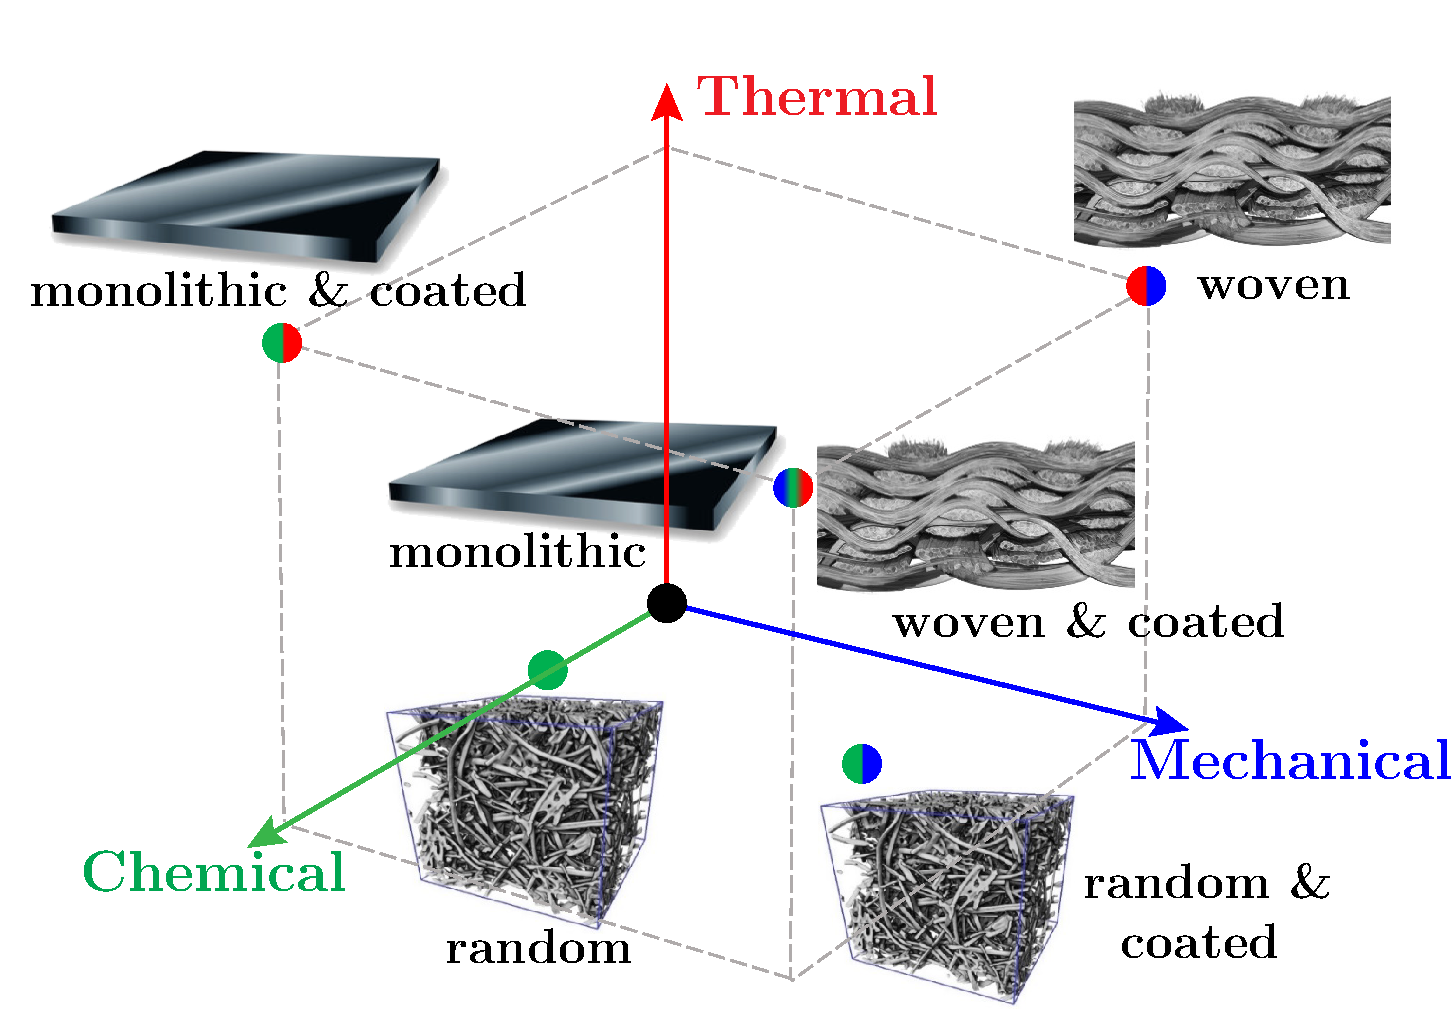
\includegraphics[width=\textwidth]{Figures/composite-design.pdf}}
%\end{minipage}
%
%\vspace*{0.2in}
%\begin{itemize}
%\setlength{\itemsep}{0.15in}
%
%\item Many-parameter design space for targeting multiple objectives
%
%\item Goal:   develop
%  and demonstrate a predictive capability
%
%\end{itemize}
%
%\end{frame}
%======================================================================




%======================================================================
%\begin{frame}\frametitle{Impact Design Cycle}
%
%\begin{itemize}
%\setlength{\itemsep}{0.2in}
%  \item \rPI{Flight Tests} expensive and inflexible:  NASA X-43A,
%    Boeing X-51A, HyShot (Queensland), HIFiRE (AFRL, AFOSR, NASA,
%    ATK-GASL,  DSTG) {\footnotesize [over last 20 years]}
%    
%   \item \rPI{Ground Tests} conditions and their evolution is a challenge,
%  and also expensive
% 
%
%  \begin{center}
%    \begin{minipage}{0.55\textwidth}
%      \begin{center}
%      \includegraphics[width=0.8\textwidth]{Figures/glass-gndtest.pdf}
%    \end{center}
%    \end{minipage}
%    \begin{minipage}{0.35\textwidth}
%      \begin{itemize}
%      \item NASA Langley DCSCTF
%      \item $M = 5$ -- $7$
%      \item Not shown:  70\,ft diameter vacuum sphere
%      \end{itemize}
%    \end{minipage}
%  \end{center}
%
%  \item Physics-based predictive simulation will accelerate design innovation
%
%\end{itemize}
%
%\end{frame}
%======================================================================




% %======================================================================
% \begin{frame}\frametitle{Scramjet:  Risk Mitigation by Predictive Science}

  
%   \begin{itemize}
%     \setlength{\itemsep}{0.4in}
%   \item Testing costs $\Rightarrow$ risk aversion:
%     \begin{itemize}
%     \item slows progress 
%     \item suppresses innovation (e.g., broad consideration of advanced materials)
%     \end{itemize}
    
%   \item Demonstrated predictive capability will 
%     \begin{itemize}
%     \setlength{\itemsep}{0.2in}
%     \item \rPI{enable discovery}:  evaluate concepts that leverage advanced materials
%     \item \rPI{prioritize}:  testing to target key
%       uncertainties and flight integration
%     \item \rPI{decrease risks}:  pre-screening of innovative novel materials
%     \end{itemize}
    
%   \end{itemize}
  
% \end{frame}
% %======================================================================


%%======================================================================
%\begin{frame}\frametitle{Model Scramjet Flame Holder}
%
%\begin{itemize}
%\item Design inspired by flight-test geometries
%\end{itemize}
%
%\raisebox{0.9in}{\fbox{\includegraphics[width=0.25\textwidth]{Figures/actii-y0-setup.pdf}}}
%\hfill
%\fbox{\includegraphics[width=0.7\textwidth]{Figures/scramjet-HIFiRE2-cavity.pdf}}
%
%
%\end{frame}
%%======================================================================

% %======================================================================
% \begin{frame}[t]\frametitle{Multi-scale/Multi-physics Challenge}


% \begin{center}
% 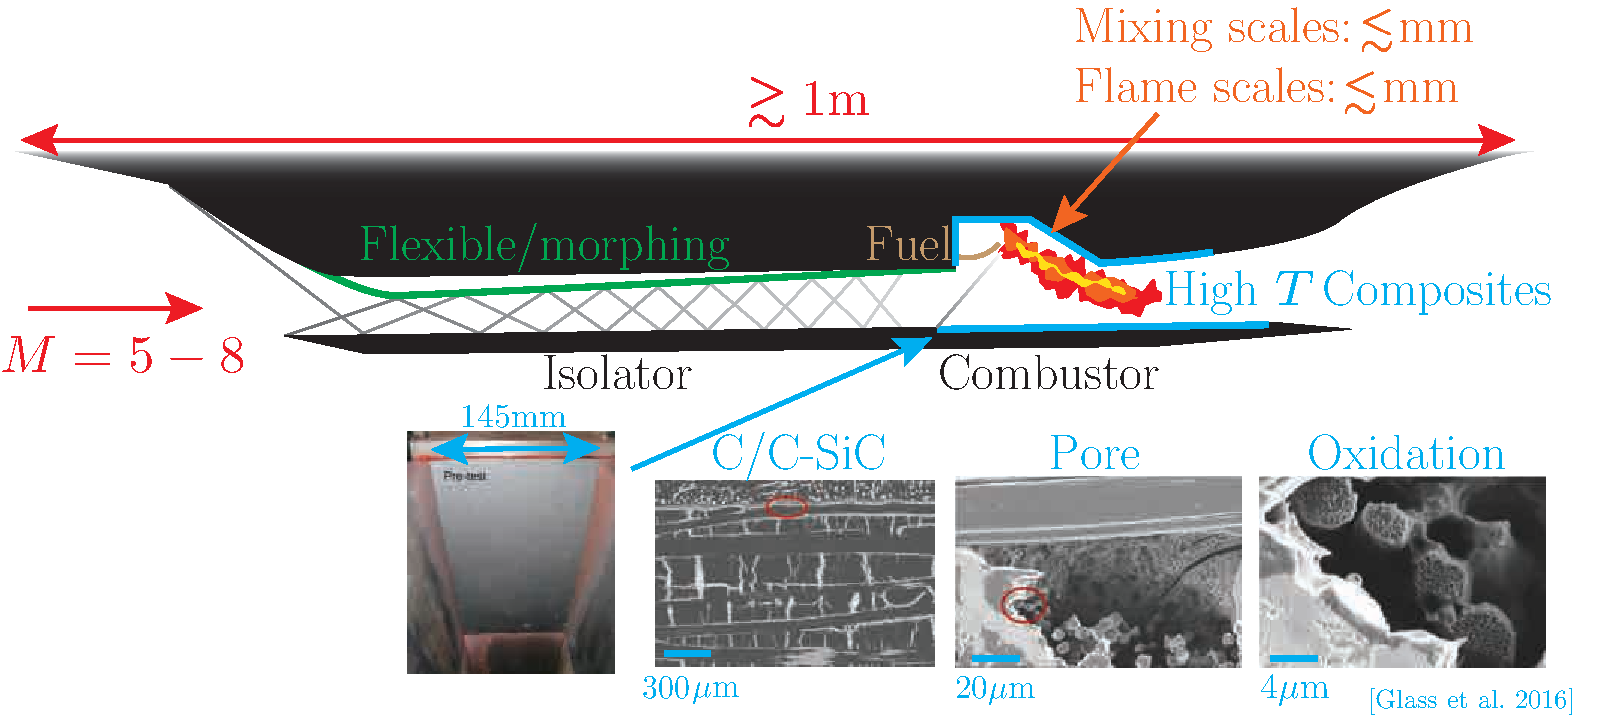
\includegraphics[width=\textwidth]{Figures/scramjet-schematic.pdf}
% \end{center}

% \onslide*<1>{
% \begin{center}
% \begin{tabular}{|ll|ll|}\hline
% Device & $\sim \mathrm{m}$ 
% & Turbulent mixing & $\lesssim \mathrm{mm}$ \\
% Flame & $\lesssim \mathrm{mm}$ 
% & Composite structure &  $\sim\mathrm{mm}$ \\
% Conduction & $\sim \mathrm{mm} - \mathrm{m}$ 
% & Mean free path & $\sim \mu\mathrm{m}$ \\
% Material defects & $\sim \mu\mathrm{m}$ 
% & Surface chemistry & $\sim \mathrm{nm}$\\\hline
% \end{tabular}
% \end{center}
% }
% \onslide*<2>{
% \begin{center}
% \begin{tabular}{|ll|}\hline
% Material degradation& $\sim \mathrm{min}$\\ 
% Thermal heating &  $\sim \mathrm{s}$ \\
% Turbulence/mixing & $\sim \mathrm{ms}$ \\
% Combustion kinetics & $\sim \mu\mathrm{s}$ \\
% Surface collisions \& phonon dynamics & $\sim \mathrm{ps}$ \\\hline
% \end{tabular}
% \end{center}
% }


% \end{frame}
% %======================================================================


%======================================================================
%\begin{frame}\frametitle{Multi-scale/Multi-physics}
%
%
%\begin{center}
%\onslide*<1>{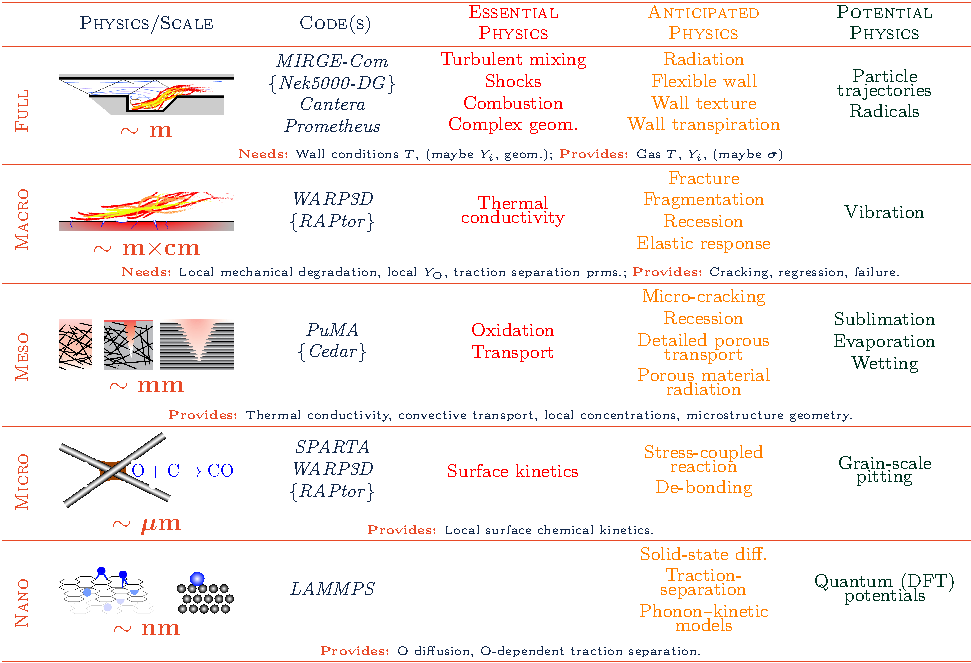
\includegraphics[width=\textwidth]{Figures/multi-physics-codes-crop.pdf}}
%\onslide*<2>{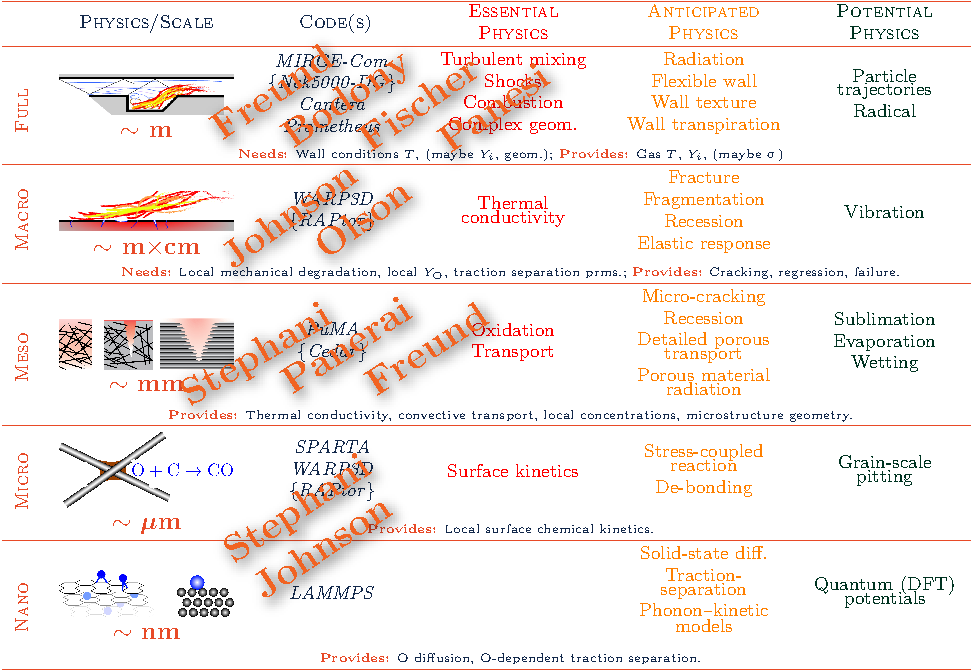
\includegraphics[width=\textwidth]{Figures/multi-physics-codes-crop-NAMES.pdf}}
%\end{center}
%
%\end{frame}
%======================================================================




%======================================================================




% \newlength{\Yhgt}
% \newlength{\Yoff}
% \setlength{\Yhgt}{0.55in}
% \setlength{\Yoff}{0.175in}

% %======================================================================
% \begin{frame}\frametitle{Annual Predictions}


% \begin{center}
% \begin{tabular}{c|c|c}\hline
% \raisebox{\Yoff}{\cPI{Y1}}
%   & \begin{minipage}[b]{1.6in}
\includegraphics[width=1.6in]{Figures/y1-schematic-isolator.pdf}\\\centerline{(post-diction)}\end{minipage}
%   & 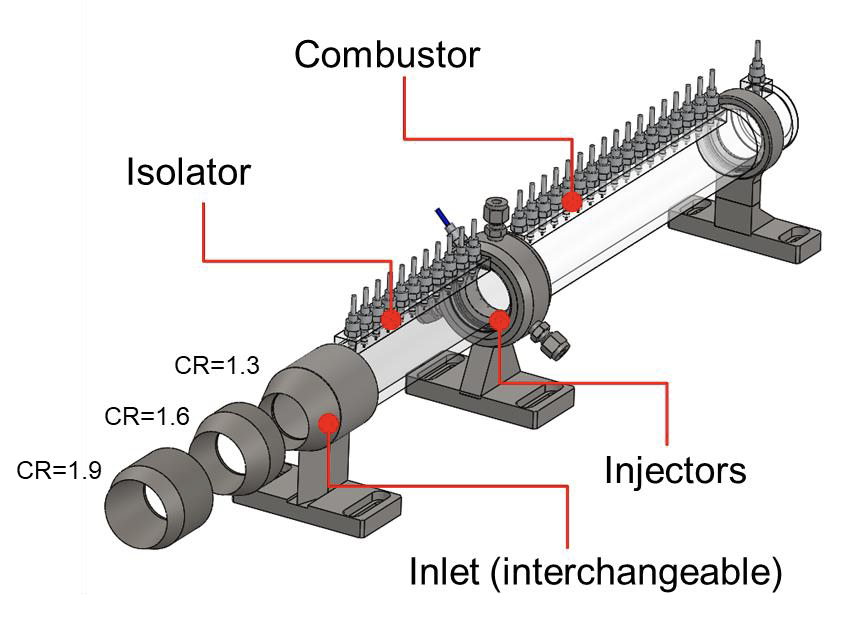
\includegraphics[height=\Yhgt]{Figures/damiano-y1-cad.png}\\\hline
% \raisebox{\Yoff}{\cPI{Y2}} 
%   & 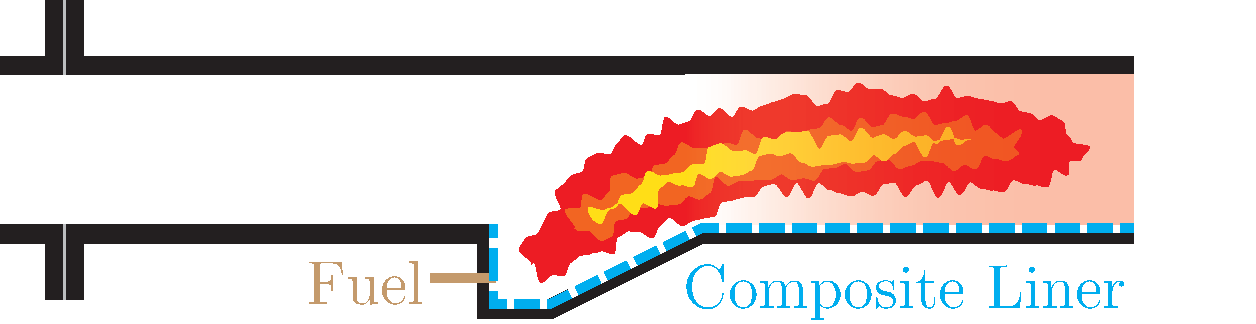
\includegraphics[width=1.6in]{Figures/y2-schematic-directconn.pdf}
%   & \includegraphics[height=\Yhgt]{Figures/actii-y0-viz.pdf}\\\hline
% \\[-0.145in]
% \raisebox{\Yoff}{\cPI{Y3}} 
%   & \raisebox{0.1in}{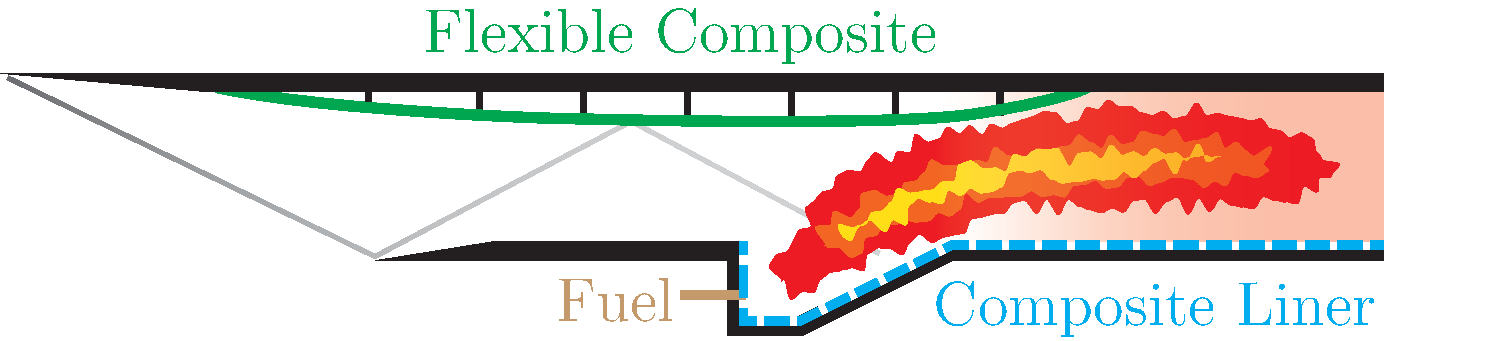
\includegraphics[width=1.6in]{Figures/y3-schematic-flight.pdf}}
%   & 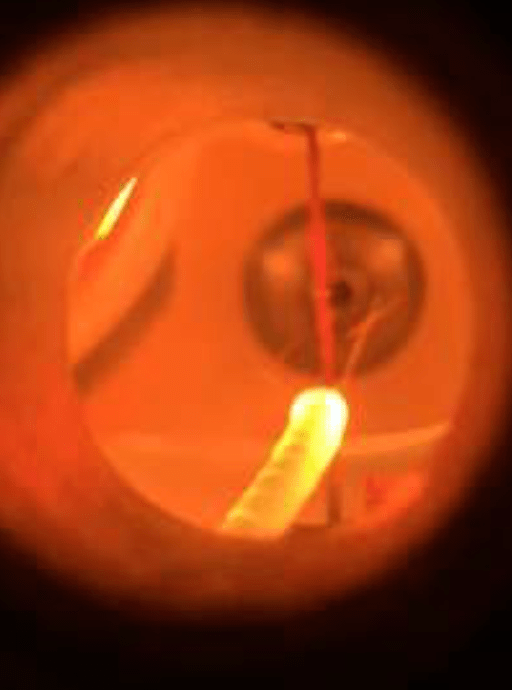
\includegraphics[height=\Yhgt]{Figures/panerai-carbon-tension.png}
% 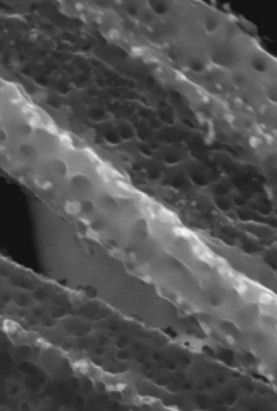
\includegraphics[height=\Yhgt]{Figures/panerai-mat-fiber.png}\\\hline
% \raisebox{\Yoff}{\cPI{Y4}} 
%   & 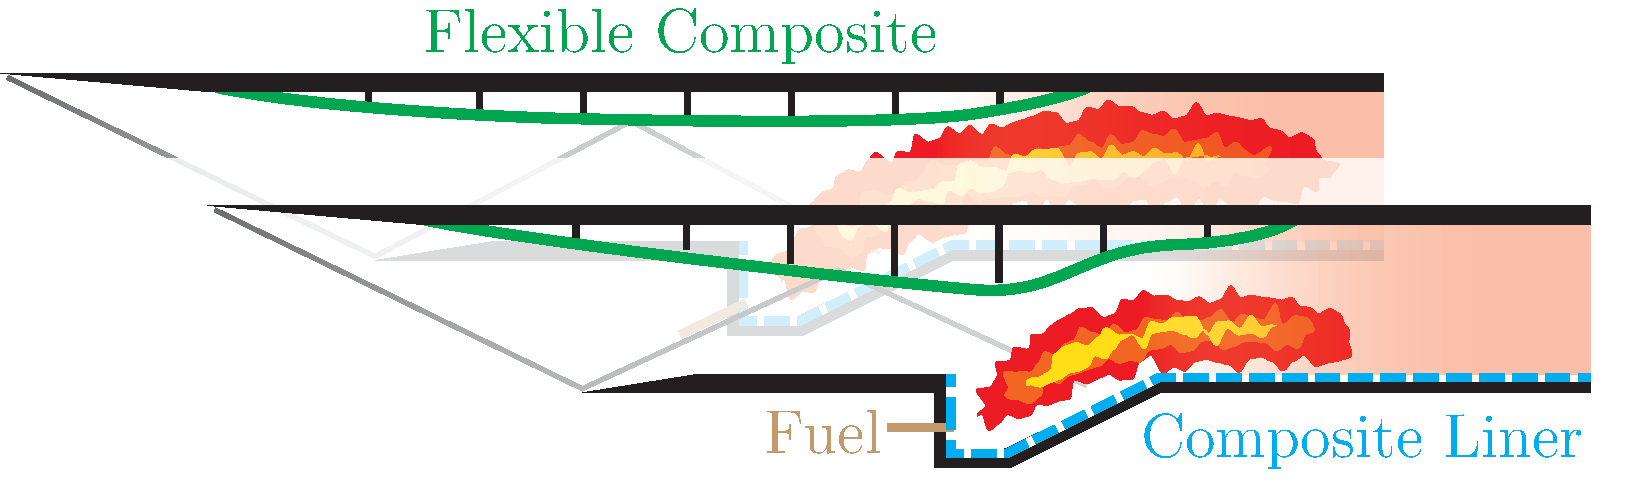
\includegraphics[width=1.6in]{Figures/y4-schematic-multiple.pdf}
%   & \includegraphics[height=\Yhgt,page=2]{Figures/timeline-sm.pdf}\\\hline
% \raisebox{\Yoff}{\cPI{Y5}} 
%   & \raisebox{0.07in}{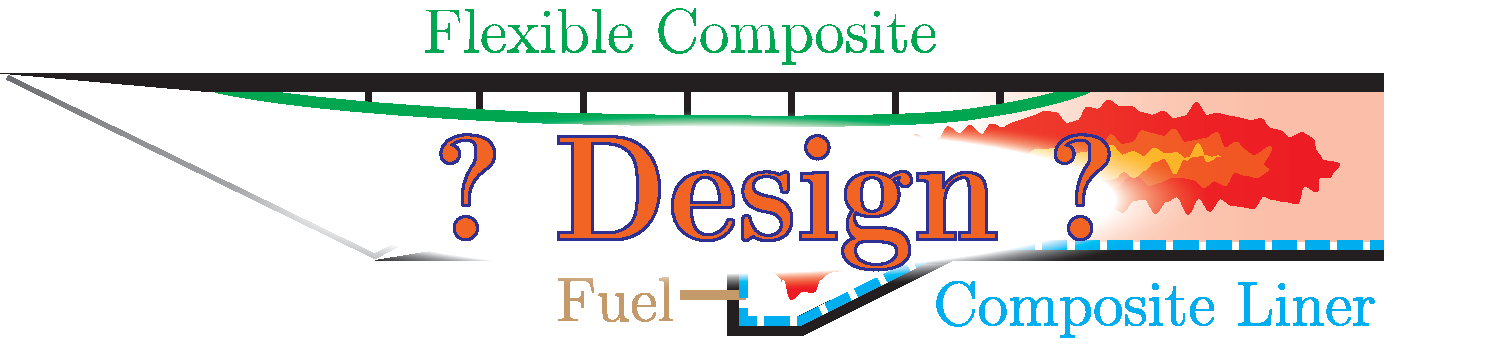
\includegraphics[width=1.6in]{Figures/y5-schematic-design.pdf}}
%   & \raisebox{-0.05in}{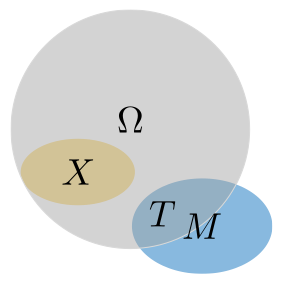
\includegraphics[height=\Yhgt]{Figures/allison-gan-venn.png}
% 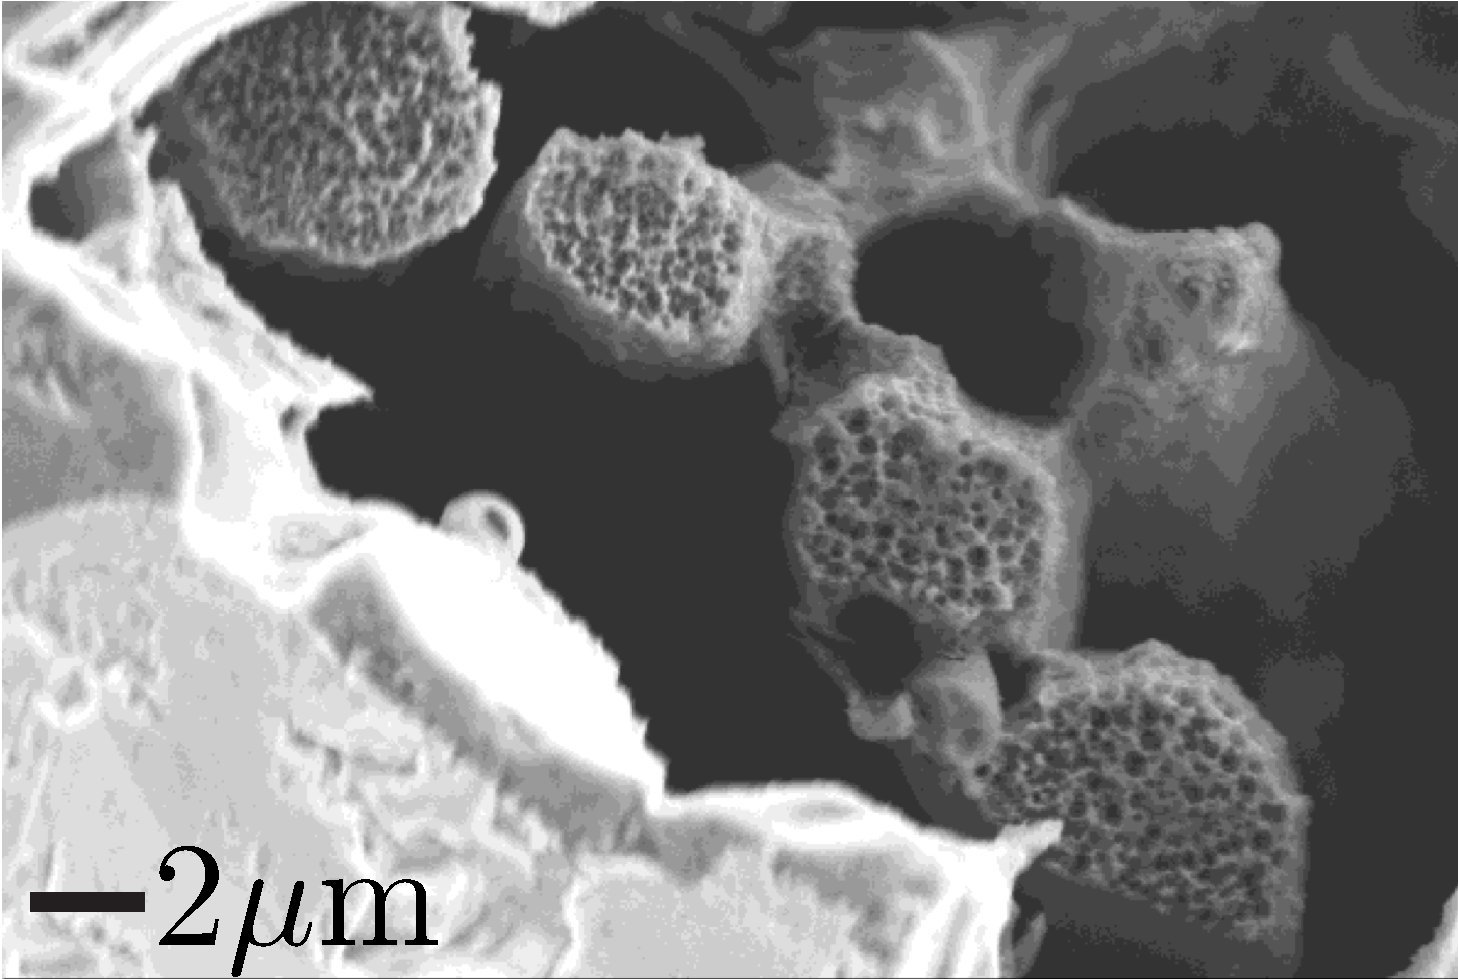
\includegraphics[height=\Yhgt]{Figures/glass-micro5.pdf}}\\\hline
% \end{tabular}
% \end{center}

% \end{frame}
% %======================================================================